\documentclass[includeheaders]{scrartcl}

\usepackage{graphicx}
\usepackage{lastpage}
\usepackage{scrlayer-scrpage}
 
\usepackage[ngerman]{babel}
\usepackage[utf8]{inputenc}

\usepackage{color}
\usepackage{tabularx}
\usepackage{float}
 \usepackage{geometry}
       \geometry{a4paper, 
             left=2.5cm, 
             right=2.5cm, 
             top=2.5cm, 
             bottom=2.5cm}

\setlength{\parindent}{10pt}
%\setlength{\headheight}{78pt}
\setkomafont{pageheadfoot}{\sffamily} 
\sloppy

\begin{document}
% o - outer, i - inner, c - center -> location of header/footer-element
%\ohead{\includegraphics[scale=0.5]{img/HPI-Logo.png}}
%\ifoot{\includegraphics[scale=0.5]{img/HPI-Logo.png} }
\ifoot{\includegraphics[scale=0.07]{img/logo}}
\cfoot{Template zur Veranstaltung Modellierung II, \\ Holger Giese, Sommersemester 2016}
\ofoot{\thepage}


\setlength{\parindent}{0pt}

% einfach diesen Teil entfernen, um nur noch eine Titelseite zu haben -->
\title{Hinweise zum Bearbeiten des Entwurfsdokuments\\ \small{(Im Rahmen der Veranstaltung Modellierung II, SoSe 2016)}
}
\date{}
\author{}
\maketitle
\textcolor{blue}{\itshape{\underline{Allgemeine Hinweise:}}}

\textcolor{blue}{\itshape{Alles, was in dieser Schriftart gesetzt ist, dient nur zur Erläuterung und sollte im fertigen Dokument nicht mehr auftauchen.}}
\\

\textcolor{blue}{\itshape{Im Dokument können (und sollen) Diagramme und verschiedene Abbildungen verwendet werden. Diagramme und Abbildungen ohne erläuternden Text sind jedoch wertlos. Bitte achten Sie daher darauf, dass jede Abbildung im Text referenziert und auch erklärt wird. Das Verhältnis zwischen erläuternden Texten und  Abbildungen sollte möglichst ausgewogen sein, d.h. ein Dokument mit 40 Seiten darf maximal 20 Seiten Abbildungen enthalten. Dieses Dokument soll insgesamt maximal 40 Seiten umfassen.}}
\\

\textcolor{blue}{\itshape{\underline{Das Template soll vollständig bearbeitet werden}}}
\\

\textcolor{blue}{\itshape{\underline{Latex-Hinweis:}}}

\textcolor{blue}{\itshape{Bilder werden folgendermaßen referenziert: In Abbildung \ref{KomponentendiagrammAbstrakt} steht ...}}

\newpage
% --> ende des zu entfernenden Teils

\newpage 

\title{Entwurfsdokument\\ \small{(Template zur Veranstaltung Modellierung II, SoSe 2016)}}
\date{}
\author{}

\maketitle

Projekt:	\textcolor{blue}{\itshape{Name des Projekts}}\\

Auftraggeber:\textcolor{blue}{\itshape{Anschrift Auftraggeber}}\\

Auftragnehmer:\textcolor{blue}{\itshape{Anschrift Auftragnehmer}}\\

\newpage

\begin{table}[h]
	\center    
    \begin{tabular}{l | l | l}
    Verantwortlichkeit & Name, Vorname & Datum \\
    \hline
    Ansprechpartner    & ~             & ~     \\
    Bearbeitender      & ~             & ~     \\
    Bearbeitender      & ~             & ~     \\
    Bearbeitender      & ~             & ~     \\
    \end{tabular}
\end{table}

\newpage
\section{Abstrakte Architektur}
\textcolor{blue}{\textit{Dieser Abschnitt beschreibt im Wesentlichen eine grobe Zerlegung der zu entwickelnden Anwendung in (Teil-)Komponenten und deren Zusammenhänge. Die Struktur der einzelnen Komponenten (also die enthaltenen Klassen und deren Beziehungen) sowie deren Schnittstellen ist nicht Teil dieser Beschreibung. Die notwendigen Schnittstellen werden erst im Laufe dieses Dokumentes entwickelt.\\\\
Die hier definierten Komponenten sind als logische Einheiten zu verstehen, die aus beliebig vielen Klassen bestehen können, die gemeinsam die Funktionalität der Komponente realisieren.\\\\
Das folgende Komponentendiagramm führt (Teil-)Komponenten ein und beschreibt ihre Abhängigkeiten.
}}

\begin{figure}[H]
\centering
\includegraphics[width=0.6\textwidth]{img/KomponentendiagrammAbstrakt.png}
\caption{\textcolor{blue}{Durch eigenes Komponentendiagramm ersetzen}}
\label{KomponentendiagrammAbstrakt}
\end{figure}

\newpage
\section{Interaktion der Komponenten}
\textcolor{blue}{\textit{Die Interaktion zwischen den Komponenten während der Ausführung eines Use Case wird durch Sequenzdiagramme (oder Interaktionsdiagramme) auf Instanzen der Komponenten (repräsentiert durch Instanzen von Schnittstellenklassen/Interfaces) beschrieben. Die dabei ver-wendeten Operationen müssen sich später in den Schnittstellen der Komponenten wiederfinden.\\\\Es müssen nicht alle Use Cases hier beschrieben werden. Stattdessen sollen nur wesentliche oder charakteristische  Use Cases  (z. B. solche, deren Ablauf bei anderen Use Cases sehr ähn-lich stattfindet) beschrieben werden.}}\\
\\
\textbf{Interaktion bei Ausführung von\\
$<$Use Cae-ID$>$: $<$Use Case-Name$>$}

\begin{figure}[H]
\centering
\includegraphics[width=0.75\textwidth]{img/SequenzDiagrammInteraktion.png}
\caption{\textcolor{blue}{Durch eigenes Sequenzdiagramm ersetzen}}
\label{SequenzDiagrammInteraktion}
\end{figure}

\newpage
\section{Komponentenschnittstellen}
\textcolor{blue}{\textit{Hier sollen die Schnittstellen der in Abschnitt 1 eingeführten Komponenten definiert werden. Des Weiteren sollen hier Nachrichten, die eventuell  über die Schnittstellen verschickt werden, definiert werden. Nachrichten sind Klassen, die beispielsweise als Parameter der in den Schnittstellen deklarierten Operationen verwendet werden.
}}

\begin{figure}[H]
\centering
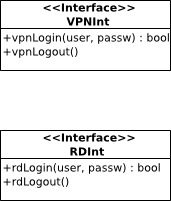
\includegraphics[width=0.3\textwidth]{img/Komponentenschnittstellen.png}
\caption{\textcolor{blue}{Durch eigenes Klassendiagramm ersetzen}}
\label{Komponentenschnittstellen}
\end{figure}

\newpage
\section{Konkrete Architektur}
\textcolor{blue}{\textit{In diesem Abschnitt werden die zuvor identifizierten Schnittstellen der Komponenten genauer beschrieben. Im Komponentendiagramm werden daher Abhängigkeiten und Implementierungsbeziehungen beschrieben bzw. ergänzt.
}}

\begin{figure}[H]
\centering

\includegraphics[width=1\textwidth]{img/KomponentendiagrammKonkret.png}
\caption{\textcolor{blue}{Durch eigenes Komponentendiagramm ersetzen}}
\label{KomponentendiagrammKonkret}
\end{figure}

\newpage
\section{Komponenten}
\textcolor{blue}{\textit{Es sollen die in der Architektur definierten Komponenten weiter beschrieben werden. Dazu ist ihre innere Struktur zu beschreiben und mit Hilfe von Klassendiagrammen, Kompositionsstrukturdiagrammen sowie Komponentendiagrammen zu modellieren. Pro Komponente sollen Parts, Ports und Konnektoren beschrieben werden. Pro Komponente sollen Klassen und Assoziationen sowie deren Methoden und Attribute definiert werden, die für die Durchführung der vorher beschriebenen Abläufe innerhalb der Komponenten benötigt werden. In den Klassendiagrammen müssen sich gegebenenfalls die in Abschnitt 4 definierten Schnittstellen wiederfinden.\\\\
Komponenten können sich während der Ausführung in verschiedenen Zuständen befinden. Sie wechseln diese, ausgelöst durch interne oder externe Ereignisse. Zustandsbezogenes Verhalten wird durch Zustandsdiagramme modelliert. Auslösende Ereignisse müssen als Operationen an den Komponentenschnittstellen zur Verfügung stehen. Ebenso sollen durch Transitionen ausgelöste Aktionen in der Komponente oder an externen Komponenten verfügbar sein.\\\\
Es muss nicht für jede Komponente ein Zustandsdiagramm erstellt werden. Zustandsdiagramme sollen nur für die Komponenten modelliert werden, die reaktiven Charakter haben und in verschiedenen Modi operieren.\\
}}

\begin{figure}[H]
\centering
\includegraphics[width=0.75\textwidth]{img/Komponenten1.png}
\caption{\textcolor{blue}{Durch eigene Diagramm ersetzen}}
\label{KomponentenStruktur1}
\end{figure}

\begin{figure}[H]
\centering
\includegraphics[width=0.85\textwidth]{img/Komponenten2.png}
\caption{\textcolor{blue}{Durch eigene Diagramm ersetzen}}
\label{KomponentenStruktur2}
\end{figure}

\begin{figure}[H]
\centering
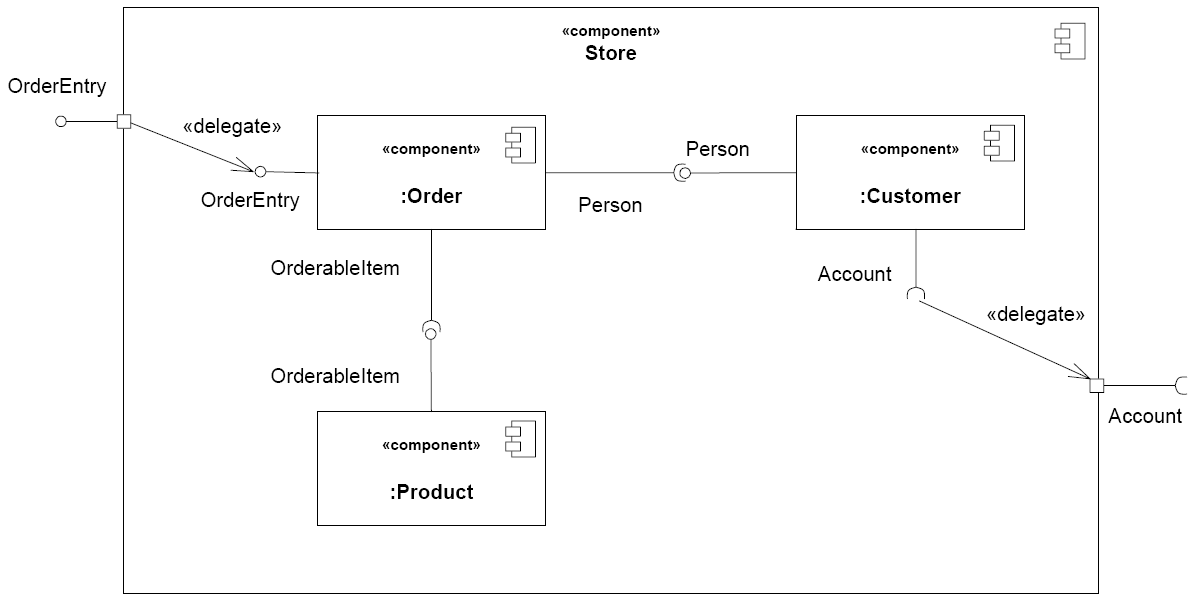
\includegraphics[width=1\textwidth]{img/Komponenten3.png}
\caption{\textcolor{blue}{Durch eigene Diagramm ersetzen}}
\label{KomponentenStruktur3}
\end{figure}

\begin{figure}[H]
\centering

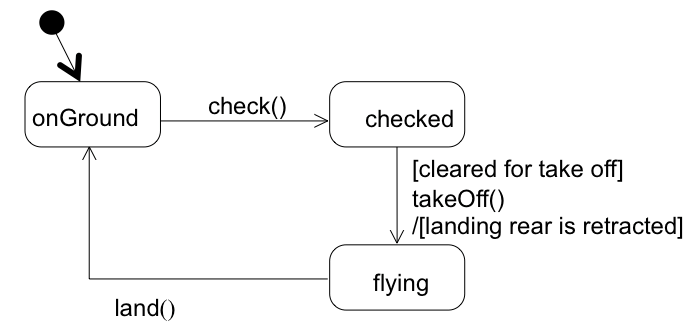
\includegraphics[width=0.6\textwidth]{img/Komponenten4.png}
\caption{\textcolor{blue}{Durch eigene Diagramm ersetzen}}
\label{KomponentenStruktur4}
\end{figure}
\newpage
\section{Paketstruktur}
\textcolor{blue}{\textit{Dieser Abschnitt beschreibt im Wesentlichen eine grobe Zerlegung der zu entwickelnden Anwendung in Pakete und deren Zusammenhänge. Dabei sollen Zusammenhänge und Abhängigkeiten zwischen den Paketen beschrieben werden.\\\\
Die hier definierten Pakete sind logische Einheiten oder gemeinsam genutzte Einheiten, die aus beliebig vielen Klassen bestehen können, welche gemeinsam die Funktionalität durch das Paket zusammenfassen. Die Aufteilung von Klassen zu Paketen muss sich dabei nicht an den strukturellen Eigenschaften der Architektur (z.B. Komponenten) orientieren. Vielmehr soll die Zerlegung in Pakete der besseren Strukturierung, Organisation, Arbeitsteilung bei Implementierung und Übersichtlichkeit der in der gesamten Architektur verwendeten Klassen dienen.\\\\
Das folgende Paketdiagramm führt Pakete ein und beschreibt ihre Abhängigkeiten. 
}}

\begin{figure}[H]
\centering
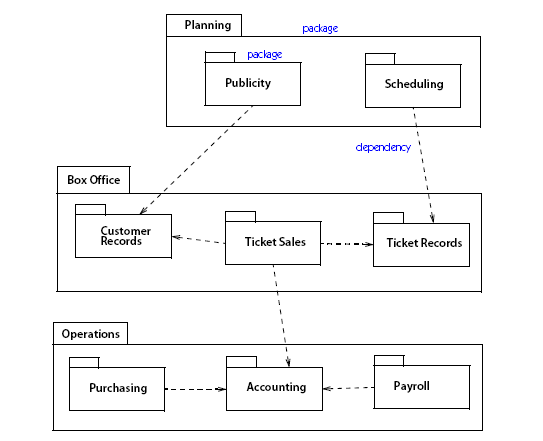
\includegraphics[width=0.8\textwidth]{img/Paketstruktur.png}
\caption{\textcolor{blue}{Durch eigene Diagramme ersetzen}}
\label{Paketstruktur}
\end{figure}

\newpage
%7
\section{Paketdetails}

%7.1 Paket Robot
\subsection{Paket \textit{Robot}}
	\begin{figure}[H]
	\centering
	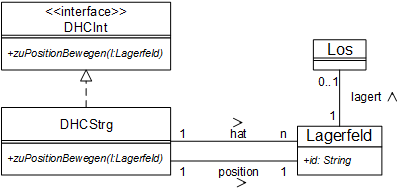
\includegraphics[width=0.6\textwidth]{../images/Paketdetails.png}
	\caption{\textcolor{blue}{HIER KOMMT DAS ROBOT - PAKETDIAGRMAM HIN}}
	\label{Paketdetails}
	\end{figure}
	Im folgenden beschreiben wir die wichtigen Klassen des Pakets \textit{Robot} 
	und ihre zugehörigen wichtigen Methoden, sowie ihre Interaktion zwischeneinander. 


	%7.1.1 RobotController
	\subsubsection{Beschreibung der Klasse \textit{RobotController}}
		\begin{figure}[H]
		\centering
		\includegraphics[width=0.6\textwidth]{../images/Iteration0_Entwurf_7-1-1_Klasse_RobotController.svg}
		\caption{\textcolor{blue}{Durch eigene Diagramme ersetzen}}
		\label{BeschreibungKlasse1}
		\end{figure}
		
		%#destination : Destination
		Die Klasse \textit{RobotController} ist die Hauptklasse des \textit{Robots}, 
		da sie den aktuellen Zustand des \textit{Robots} enthält.
		So hat diese Klasse die Möglichkeit höchstens eine \textit{Destination} zu speichern. 
		Diese \textit{Destination} kann ein vom \textit{Server} zugeteiltes Ziel sein, 
		der dem \textit{Robot} zugehörige \textit{Charger}, oder gerade kein Ziel, 
		also \textit{null} sein. Nur wenn der \textit{Robot} gerade keine \textit{Destination} 
		gespeichert hat, kann er neue Aufträge vom \textit{Server} annehmen.

			%7.1.1.1 #collectSensorData():void
			\subsubsubsection{Beschreibung der Methode \textit{collectSensorData}}
			Die Methode \textit{collectSensorData} wird von der Methode \textit{recieveMessage} 
			aus der Klasse \textit{RobotCommunication} aufgerufen, wenn eine Neue \textit{Message} 
			vom Server eingegangen ist, welche den \textit{Robot} dazu auffordert, Informationen 
			über seinen Zustand zu senden. Der \textit{Robot} fragt dann seine Hardwareschnittstelle 
			nach seiner Position und seinem Akkustand an, und verfasst eine neue \textit{Message} 
			die diese Informationen, sowie seinen Aktuellen Zustand bzw. seine aktuelle \textit{Destination} enthalten.

	%7.1.2 DrivingSystem
	\subsubsection{Beschreibung der Klasse \textit{DrivingSystem}}
		\begin{figure}[H]
		\centering
		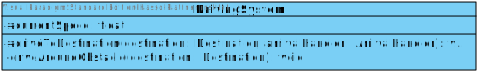
\includegraphics[width=0.6\textwidth]{../images/Iteration0_Entwurf_7-1-2_Klasse_DrivingSystem.svg}
		\caption{\textcolor{blue}{Durch eigene Diagramme ersetzen}}
		\label{BeschreibungKlasse1}
		\end{figure}
		
		%#currentSpeed:float
		Diese Klasse beschreibt den aktuellen Zustand des Fahrsystems des \textit{Robots}. 
		Es sind Informationen über die aktuelle Geschwindigkeit enthalten und die Methode, 
		die gerade ausgeführt wird, gibt Auskunft über die aktuelle Beschäftigung des \textit{Robots}.

			%7.1.2.1 	#driveToDestination(destination: Destination, arrivalHandler: ArrivalHandler): void
			\subsubsubsection{Beschreibung der Methode \textit{driveToDestination}}
			\begin{figure}[H]
			\centering
			\includegraphics[width=0.6\textwidth]{../images/Iteration0_Entwurf_7-1-2-1_Methode_driveToDestination.svg}
			\caption{\textcolor{blue}{Durch eigene Diagramme ersetzen}}
			\label{BeschreibungKlasse1}
			\end{figure}

			Wenn diese Methode aufgerufen wird, macht der \textit{Robot} sich auf den Weg zur 
			übergebenen \textit{Destination}. Wenn der \textit{Robot} an dieser \textit{Destination} 
			angekommen ist, wird die Methode des übergebenen \textit{ArrivalHandlers} ausgeführt. 
			Wenn sich ein \textit{Obstacle} auf dem Weg befindet, wird die Methode \textit{driveAroundObstacle} 
			aufgerufen, bis das \textit{Obstacle} umfahren wurde.

			%7.1.2.2    -driveAroundObstacle(destination: Destination): void
			\subsubsubsection{Beschreibung der Methode \textit{driveAroundObstacle}}
			\begin{figure}[H]
			\centering
			%TODO: Sequenzdiagramm
			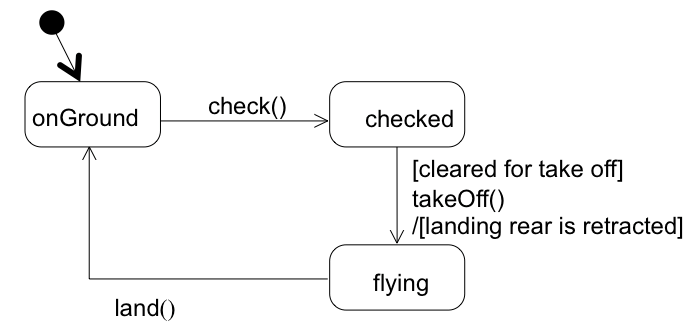
\includegraphics[width=0.6\textwidth]{img/BeschreibungKlasse1.png}
			\caption{\textcolor{blue}{Durch eigene Diagramme ersetzen}}
			\label{BeschreibungKlasse1}
			\end{figure}

			Diese Methode wird von \textit{driveToDestination} mit des Position eines \textit{Obstacles} aufgerufen, 
			wenn ein \textit{Obstacle} zu umfahren ist.
			Dabei entscheidet sich der Roboter zunächst ob er links oder rechts an dem \textit{Obstacle} vorbeifährt, 
			und hält sich dann mithilfe seiner Sensoren immer auf einem bestimmten Abstand zum Hindernis, bis zwischen 
			\textit{Obstacle} und der Luftlinie zur \textit{Destination} genug Platz für den \textit{Robot} ist.
	
	%7.1.3 RobotCommunication
	\subsubsection{Beschreibung der Klasse \textit{RobotCommunication}}
		\begin{figure}[H]
		\centering
		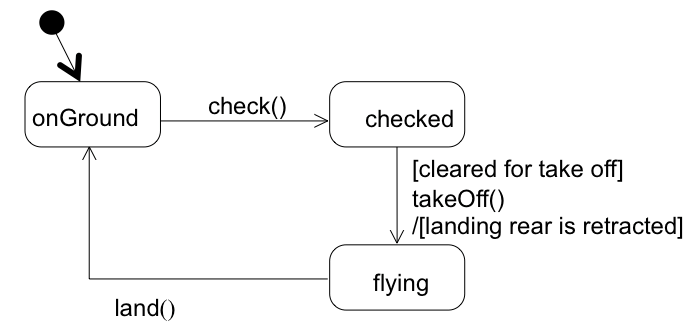
\includegraphics[width=0.6\textwidth]{img/BeschreibungKlasse1.png}
		\caption{\textcolor{blue}{Durch eigene Diagramme ersetzen}}
		\label{BeschreibungKlasse1}
		\end{figure}
		%	-communicationID: int
		
			%7.1.3.1	#sendMessage(m: Mesasage): void
			\subsubsubsection{Beschreibung der Methode \textit{sendMessage}}
	
			%7.1.3.2	#receiveMessage(): void
			\subsubsubsection{Beschreibung der Methode \textit{receiveMessage}}
	

	\begin{figure}[H]
	\centering
	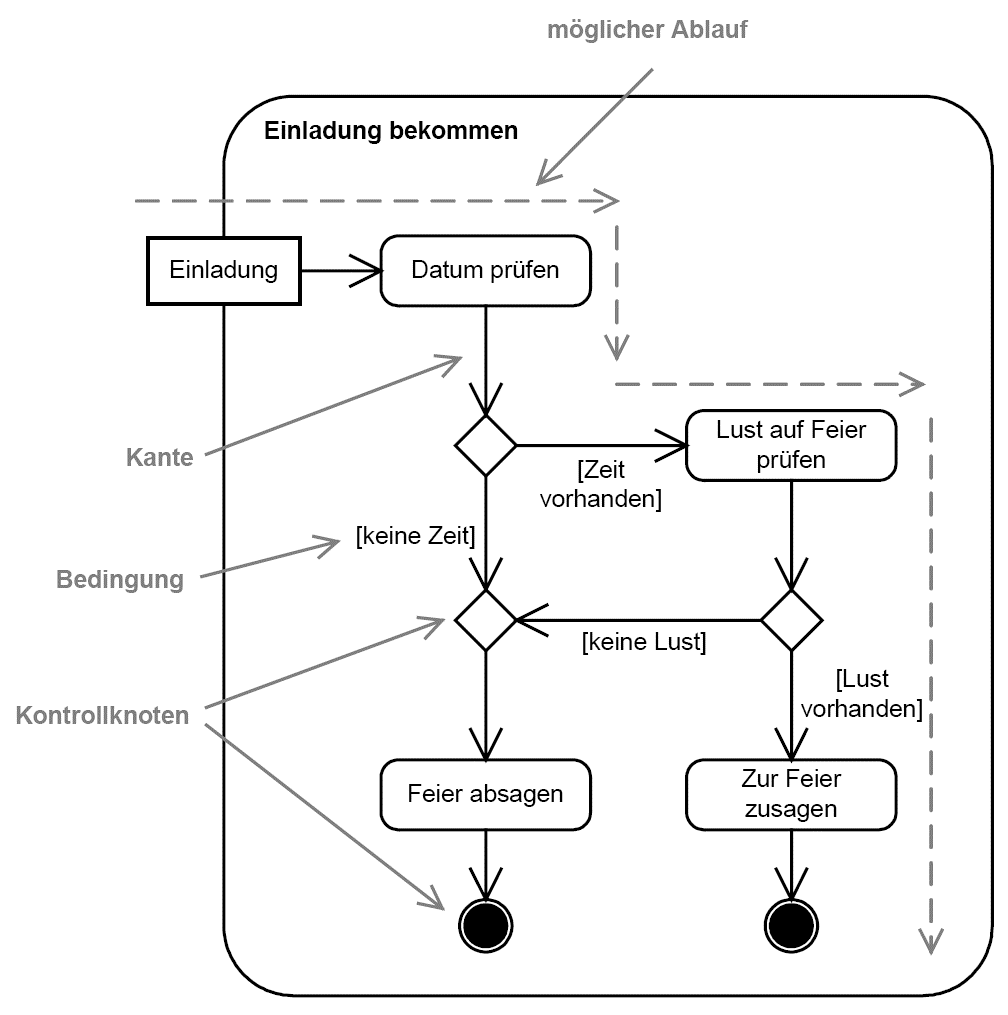
\includegraphics[width=0.6\textwidth]{img/BeschreibungKlasse2.png}
	\caption{\textcolor{blue}{Durch eigene Diagramme ersetzen}}
	\label{BeschreibungKlasse2}
	\end{figure}

\newpage
\section{Abläufe}
\textcolor{blue}{\textit{Wesentliche Abläufe innerhalb des Produkts oder innerhalb von Paketen sollen weiter verfeinert werden. Dabei sind gegebenenfalls die Abläufe auf Komponentenebene zu verfeinern sowie das interne Verhalten umzusetzen.\\\\
Dabei kann es sich um Abläufe handeln, welche Use Cases entsprechen oder von Objekten einer Klasse selber angestoßen werden (z. B.  bei aktiven Klassen). \\\\
Die Modellierung kann mit Hilfe von Interaktionsdiagrammen unter Berücksichtigung der in vorangehenden Abschnitten definierten inneren Struktur erfolgen. \\\\
Bei der Erstellung der Interaktionen sollen folgende Eigenschaften gelten. Die Rollen der modellierten Interaktionen müssen in den Strukturen vorhanden sein, die verwendeten Operationen der Nachrichten müssen in der zugehörigen Klasse, bzw. Schnittstelle spezifiziert sein, die Interaktion muss mit einem evtl. angegebenen Lebenszyklus (siehe Abschnitt 7.1) zusammenspielen und die umgesetzten Interaktionen sollen Use Cases, bzw. Abläufen auf Komponentenebene entsprechen.
}}

\textbf{Interaktion \textcolor{blue}{$<$kurzer Titel$>$}}\\
\textit{\textcolor{blue}{oder}}\\
\textbf{Interaktion bei Ausführung von \textcolor{blue}{$<$Use Case-ID$>$: $<$Use Case-Name$>$}}\\

\begin{figure}[H]
\centering
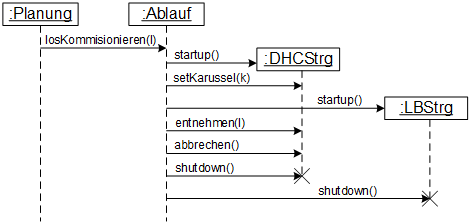
\includegraphics[width=0.75\textwidth]{img/Interaktion1.png}
\caption{\textcolor{blue}{Durch eigene Diagramm ersetzen}}
\label{Interaktion1}
\end{figure}

\newpage
\section{Produkteinsatz}
\textcolor{blue}{\textit{In diesem Abschnitt wird der geplante Einsatz des zu entwickelnden Produktes beschrieben. Dies umfasst insbesondere die Systemumgebung in der das Produkt eingesetzt werden soll und die Zuordnung der Software zu dieser.
}}

\begin{figure}[H]
\centering
\includegraphics[width=0.75\textwidth]{img/Produkteinsatz.png}
\caption{\textcolor{blue}{Durch eigene Diagramme ersetzen}}
\label{Produkteinsatz}
\end{figure}


\end{document}
